\newpage

\section{Getting Started with the CPX/CPB}\label{s:Getting_Started}

\subsection{Parts List}
\begin{enumerate}[itemsep=-5pt]
  \item Laptop
  \item CPX(or CPB)
  \item USB Cable (with a data line. Not all USB cables have data
    lines)
\end{enumerate}

\subsection{Setting up your Circuit Playground}

By now you hopefully have your Circuit Playground (CPX) and it's time
to get your CPX up and running. A very in depth and detailed tutorial
can be found on the
\href{https://learn.adafruit.com/circuitpython-made-easy-on-circuit-playground-express/first-things-first}{Adafruit
  Learn site.} The text below is a summary 
of what you need to do to get the CPX up and running. 

When you get your CPX and plug it into the computer via USB it
actually won't run Python just yet. First you need to double click the
reset button (the button in the center. It says RESET above the
button) and put it into boot mode. All the neopixels (the ring lights
on the CPX) will light up green. 
\begin{figure}[H]
  \begin{center}
    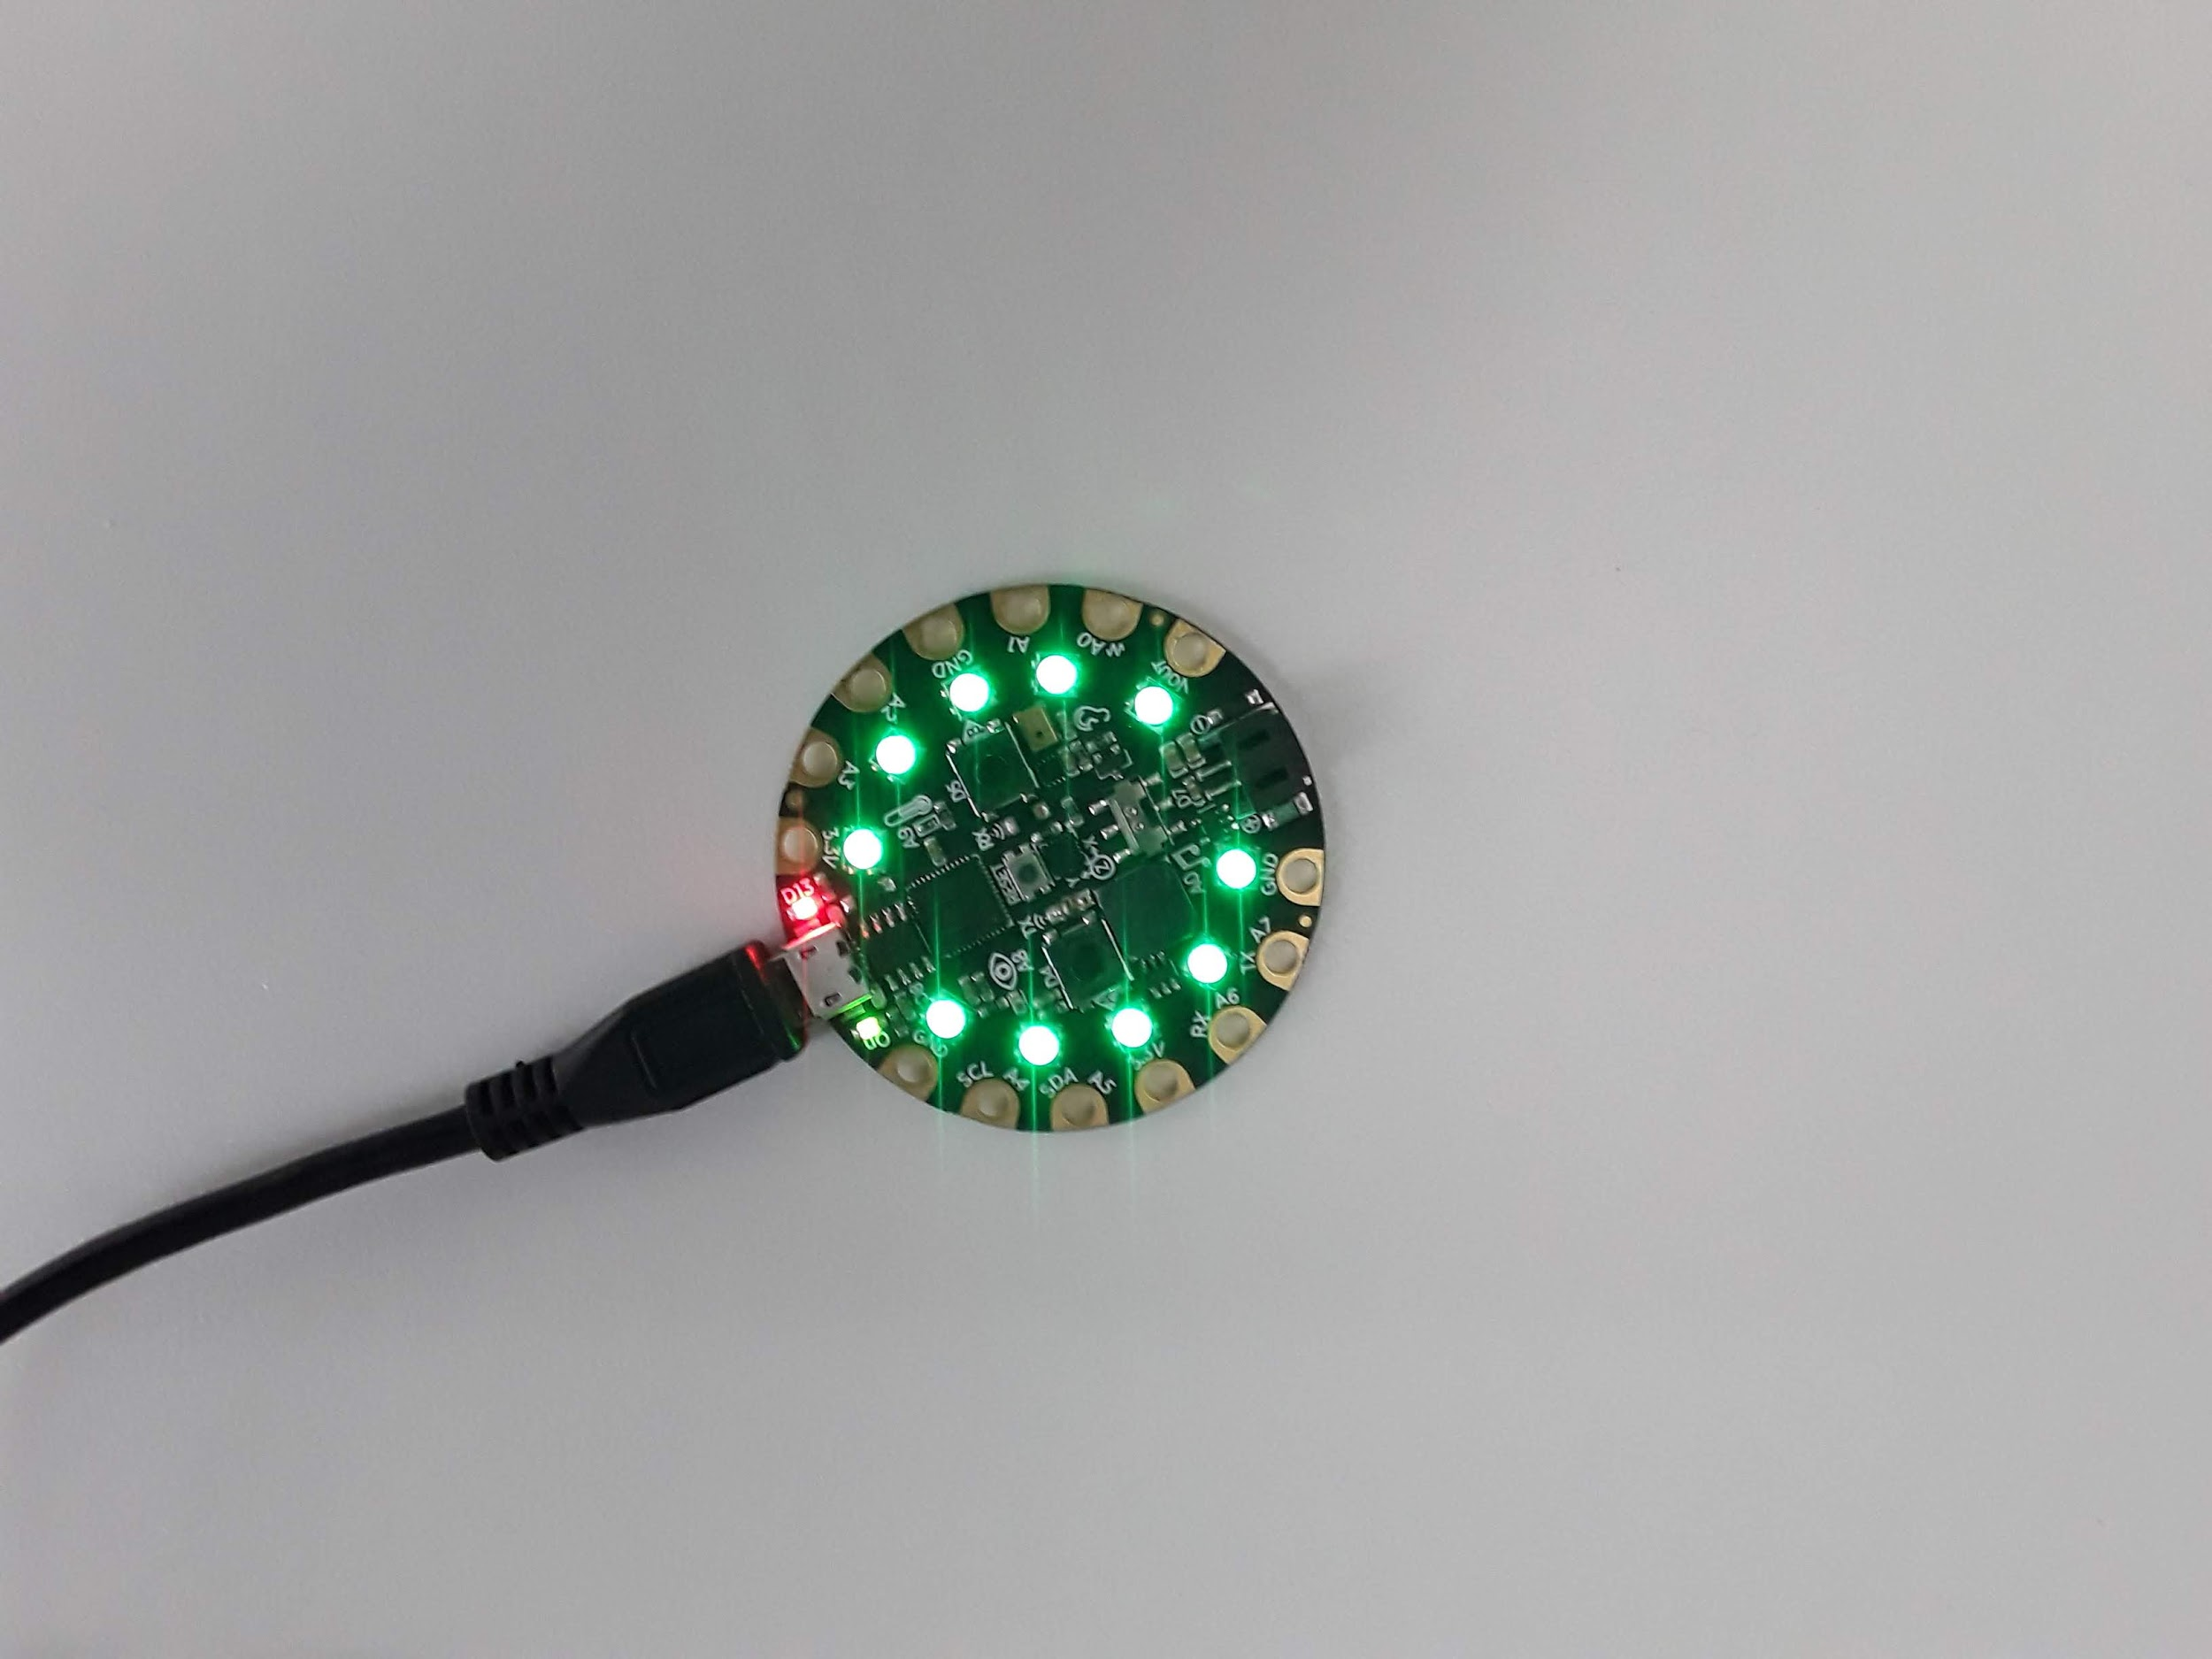
\includegraphics[width=\textwidth]{Figures/CPX_boot.jpeg}
  \end{center}
\end{figure}
Something called CPLAYBOOT will pop up on your computer just like a
USB stick or external harddrive. A couple files with be in there but
it doesn’t matter what they say right now.
\begin{figure}[H]
  \begin{center}
    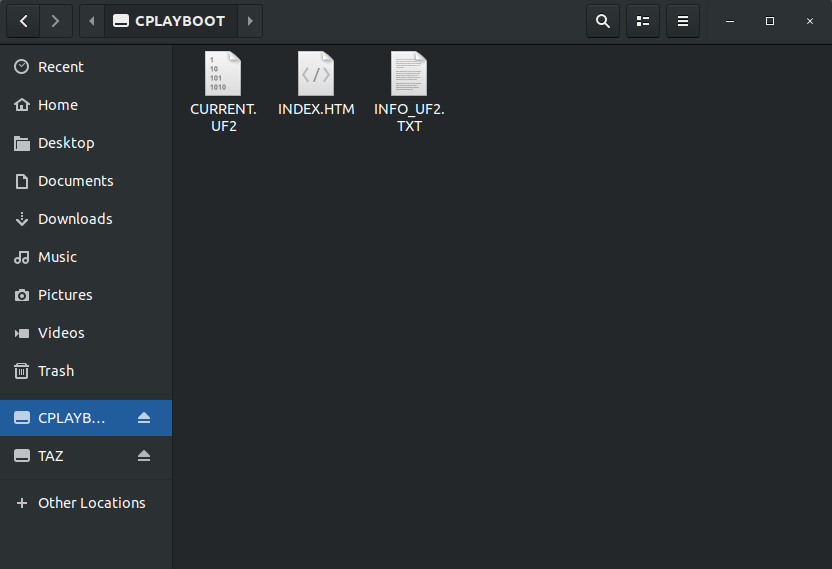
\includegraphics[width=\textwidth]{Figures/CPLAYBOOT.png}
  \end{center}
\end{figure}
You then need to download what’s called a \href{https://circuitpython.org/board/circuitplayground_express/}{UF2 file} and transfer it
onto the CPX. Note if you purchased a kit with the Bluefruit you need
to download a
\href{https://circuitpython.org/board/circuitplayground_bluefruit/}{different
  UF2}. Make sure you get the right one. Once the 
UF2 is downloaded you need to drag the UF2 over to the CPLAYBOOT drive
on your computer. After a bit of time a USB drive called CIRCUITPY
will pop up as a flash drive on your computer. The CPX is now like a
USB stick with 2MB of storage. {\bf Note that if you have an old bootloader you must update the \href{https://learn.adafruit.com/adafruit-circuit-playground-bluefruit/update-bootloader-use-command-line}{bootloader}.}
\begin{figure}[H]
  \begin{center}
    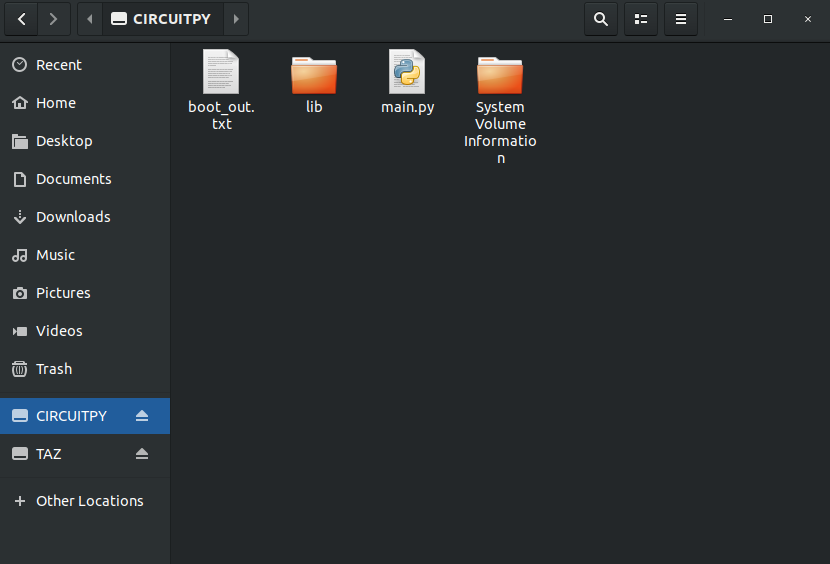
\includegraphics[width=\textwidth]{Figures/CIRCUITPY.png}
  \end{center}
\end{figure}
At this point the CPX is like a mini computer. If you put Python code
on the “flash drive” it will run python code. Since I’ve done this
before, there are a number of files already on my CPX. You may have
some or none of these. The “boot\_out.txt” file will tell you the
version of CircuitPython you have on the CPX. Mine says this:
\begin{verbatim}
Adafruit CircuitPython 5.3.0 on 2020-04-29; Adafruit CircuitPlayground Express with samd21g18
\end{verbatim}
Which means I have CircuitPython version 5.3.0 last updated on April
29th, 2020. The CPX itself is using the \href{https://www.microchip.com/wwwproducts/en/ATsamd21g18}{ATSAMD21G18}
microprocessor. The folder lib is a folder with extra libraries that
you may need to install later. The file main.py is the Python file
that the CPX is currently running. {\bf The CPX can store as many Python
files as possible for a 2MB flash drive but it will only run ONE
Python script at a time and that file must be named main.py} The folder
{\it System\_Volume\_Information} is a file management folder that we will
never use.

If you want the CPX to run code you simply need to edit the file
{\it main.py} or if that file does not exist you just need to create it. You
could just open Notepad or any other text app (Sublime,TexWrangler,
Emacs, Vi, Nano, Gedit, Notepad++, Wordpad, VSCode, etc) but the CPX
has alot of debugging options and it is recommended to use a program
called “\href{https://codewith.mu/en/download}{Mu}”. Mus is a good way to write and debug code on the
CPX. Note that Mu is only used to program the CPX. If you want to run
Python code on your laptop you need to use Thonny or Spyder (or
whatever other IDE you downloaded). If you want to run Python code on
your CPX you must use Mu. Once you’ve downloaded and installed Mu and
open it up it will look like this (Note it's possible the the software
gets updated from the time this book is published. As such be sure to
select the Circuitpython Mode for board development).
\begin{figure}[H]
  \begin{center}
    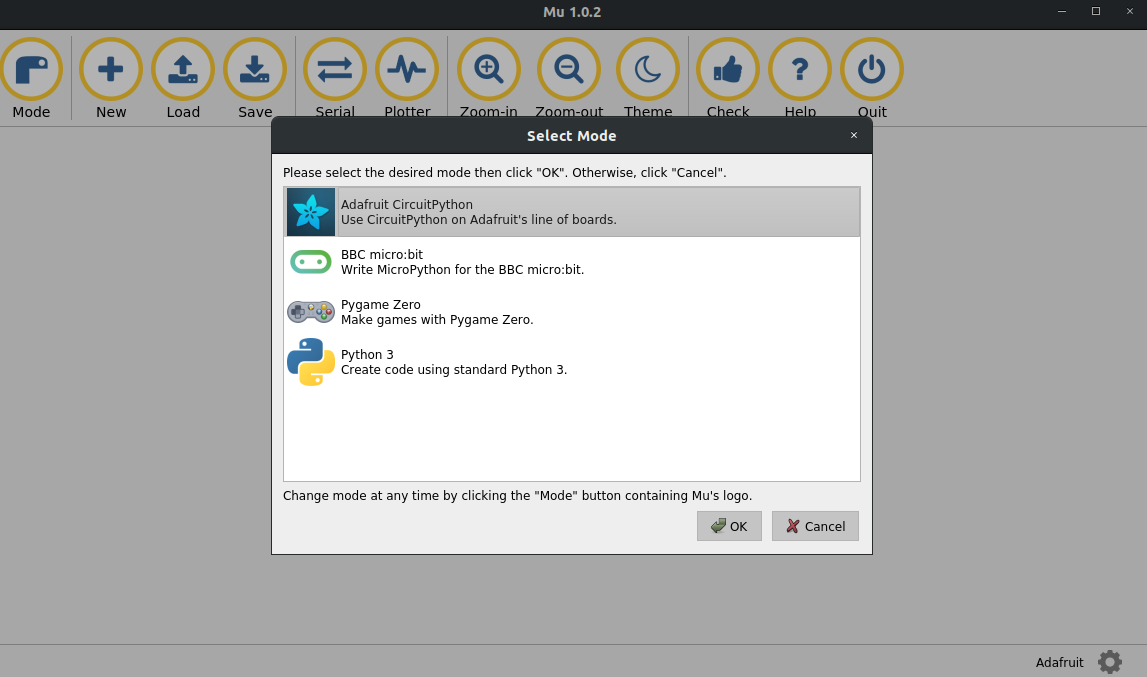
\includegraphics[width=\textwidth]{Figures/Mu.png}
  \end{center}
\end{figure}
Make sure to select the “Adafruit CircuitPython” option. If the
software has been updated and that option no longer exists, be sure to
select the option that says Circuitpython for board development.

Alright, let’s start writing code! If you have a file called {\it main.py}
on your CPX click the Load button and load {\it main.py} (make sure to load
the main.py that is stored on your CPX and not somewhere else on your
computer.) If a file {\it main.py} does not exist on your CPX simply click
the New button and then Save the file as {\it main.py} (again make sure you
save it to the CPX and not to your computer) 
\begin{figure}[H]
  \begin{center}
    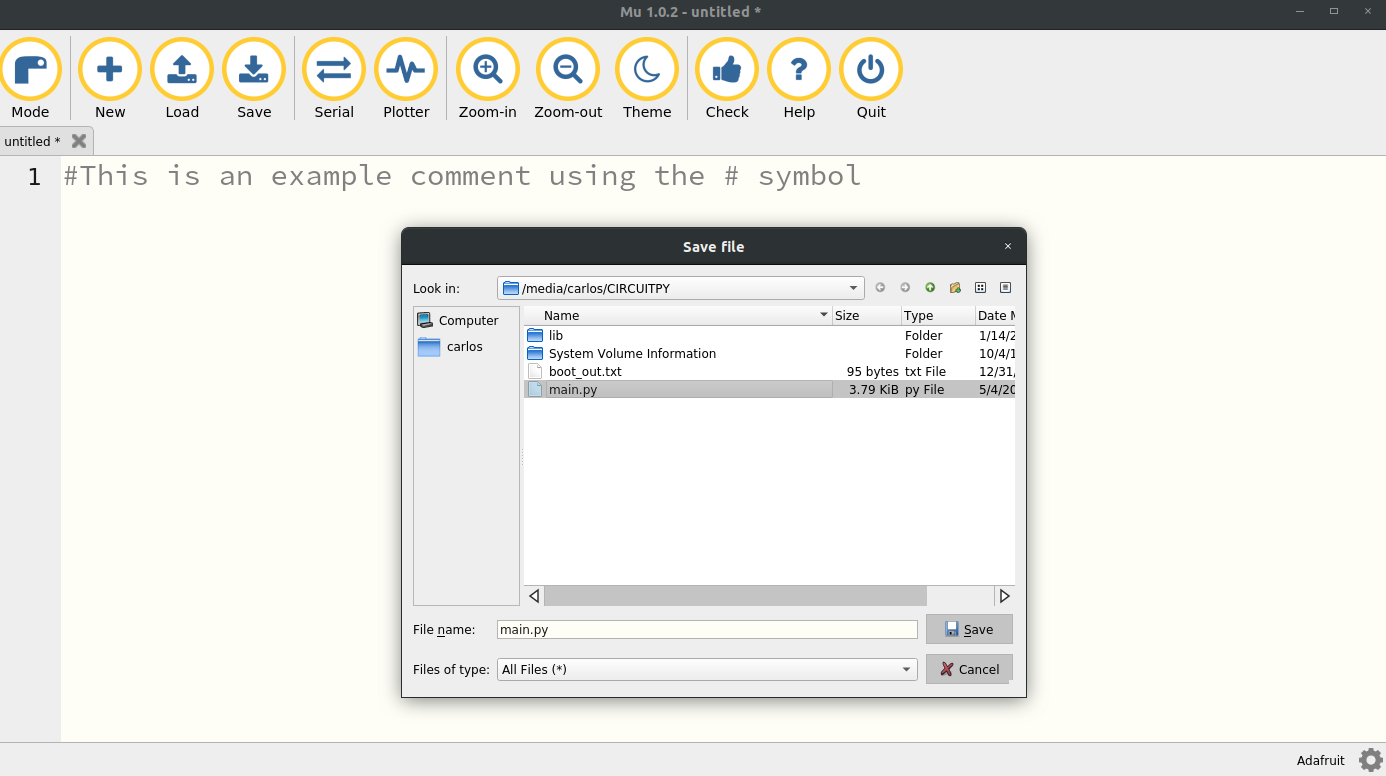
\includegraphics[width=\textwidth]{Figures/Mu2.png}
  \end{center}
\end{figure}
You’ll see that I am accessing the CIRCUITPY drive and saving the file
as main.py The file itself is empty and just has a comment using the \#
symbol. At this point since the file is blank the CPX won’t do
anything.

{\bf \it Now this is really important. Your CPX is a USB stick that can hold as
many Python files as 2MB will allow but it can only run or execute one
python script at a time. Furthermore it will only run two types of
files. It will run code.py if it exists and if it can't find code.py
it will run main.py If the CPX can't find main.py or code.y it will
just not do anything. If you have two versions of main.py or a
combination of main.py or code.py it will run one of them and not the
other. Make sure you only have one version of main.py or code.by but
not both! Some common things to check if your CPX isn't working. }
\begin{enumerate}[itemsep=-5pt]
  \item Make sure you're using Mu in the right Mode
  \item Make sure main.py or code.py is on the CIRCUITPY drive and not somewhere on your computer.
  \item Make sure you are editing the right file in Mu. Do you have two versions of main.py?
  \item Are you editing using Thonny or Spyder?
  \item Are you editing a file on your computer? Make sure you are writing to the CIRCUITPY drive.
  \item Unplug the CPX, close Mu and try again.
\end{enumerate}
So let’s get the CPX to do something simple like blink an LED. I have
an entire
\href{https://github.com/cmontalvo251/Microcontrollers}{Github}
devoted to Microelectronics. Specifically I have a
\href{https://github.com/cmontalvo251/Microcontrollers/tree/master/Circuit_Playground/CircuitPython}{folder
  with all of my Circuit Playground files}. The easiest program to 
run is the \href{https://github.com/cmontalvo251/Microcontrollers/blob/master/Circuit_Playground/CircuitPython/blink.py}{blink.py} script. I’ve attached a screenshot of the script
below. 
\begin{figure}[H]
  \begin{center}
    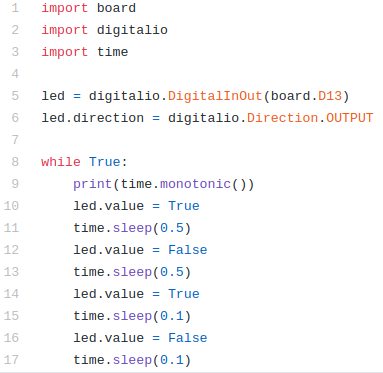
\includegraphics[width=\textwidth]{Figures/blink.png}
  \end{center}
\end{figure}
We will talk about what this code is doing later on. For now copy and
paste these 17 or so lines of code and paste them into Mu specifically
the {\it main.py} script. It will hopefully look like this.
\begin{figure}[H]
  \begin{center}
    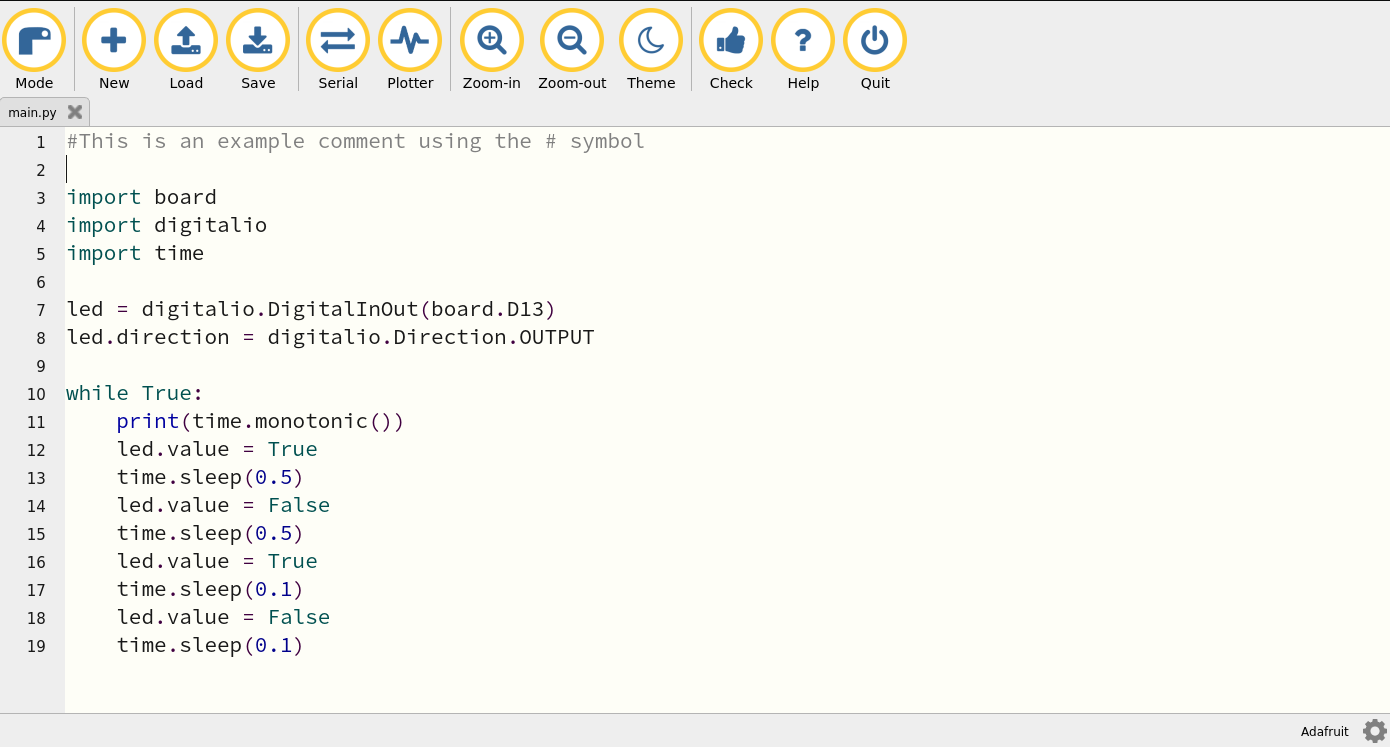
\includegraphics[width=\textwidth]{Figures/blinkmu.png}
  \end{center}
\end{figure}
Make sure to save. You can click {\it Zoom-In} and {\it Zoom-out} to zoom in and
out to change the font size and see more of the output. If the blink
code is working you will see a red led labeled D13 on the CPX blink
back and forth. D13 stands for digital pin 13. You’ll notice there are
analog pins labeled A5 and A6 among other numbers. Let’s talk about
the code a bit more and explain why it’s doing what it’s doing. The
three lines at the top of the code are {\it import} commands to import
different modules just like we did for {\it numpy} and {\it matplotlib}. In this
case the modules being imported are {\it board}, {\it digitalio} and
{\it time}. The module {\it board} is used to import the layout of the
CPX so we can access different pins on the CPX. The module {\it digitalio}
stands for digital input output which means we are inputting and
outputting digital signals. Since we can combine this module with the
{\it board} module we will be able to output digital signals to
different pins on the CPX board. Remember that PCB stands for printed
circuit board so {\it board} implies we are accessing pins on the CPX
PCB. Hopefully that makes sense. The final module we are importing is
{\it time} which acts just like the {\it time} module on your desktop
computer. It will let us access the CPX’s internal clock.

Moving along, lines 7 and 8 create an LED object using the {\it board}
module and {\it digitalio}. It’s a long line of code that basically says,
create a variable called {\it led} that lets us output a digital signal to
pin D13. We also set the direction of the LED to output since we only
want to write to the LED.

Lines 10 through 19 kick off an infinite loop that never ends. The
line that says {\it while True:} means loop while {\it True}. Well
{\it True} is always true which means it will loop forever. The colon
at the end of the line tells Python that the loop condition statement
ends and to begin looping from 11 through 19.

Line 11 specifically says {\it print(time.monotonic())}. First the
{\it print()} function is used to print things so that you and I can
see it. Rather than just seeing a blinking LED we want to see the time
printed. The {\it time.monotonic()} is using the module {\it time} which we
imported and using a function from that module called {\it monotonic()}
which calls the internal clock of the CPX. So how do you see the
output from the print statement? Hit the {\it Serial} button on Mu and you
will hopefully see some output. Here’s what it looks like on my
machine. 
\begin{figure}[H]
  \begin{center}
    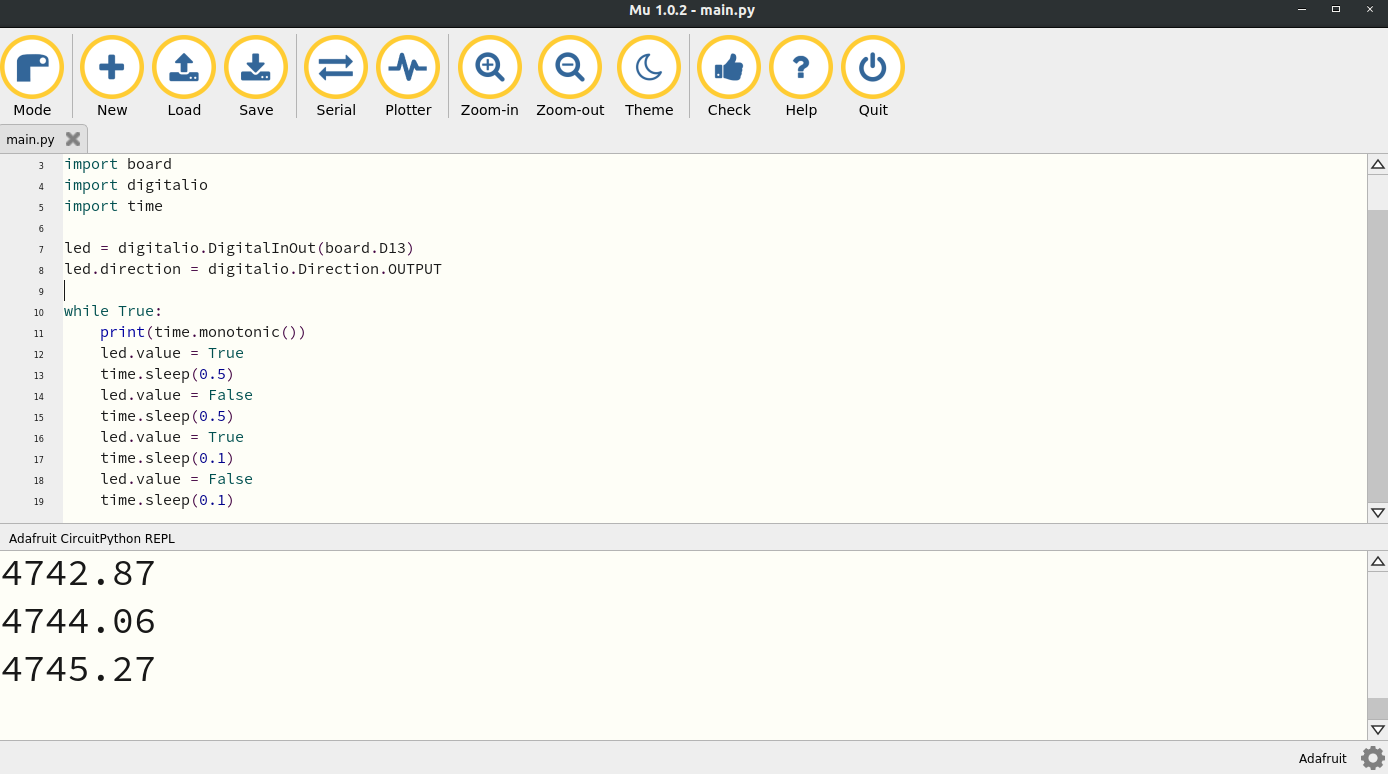
\includegraphics[width=\textwidth]{Figures/blinkmu2.png}
  \end{center}
\end{figure}
In this case you can see the time printed every time it goes through
the loop. You may even see an error. This {\it Serial} button is great for
debugging because it will tell you the error in your code. For
example, in the picture below I have an error in my code and the
{\it Serial} output is letting me know.
\begin{figure}[H]
  \begin{center}
    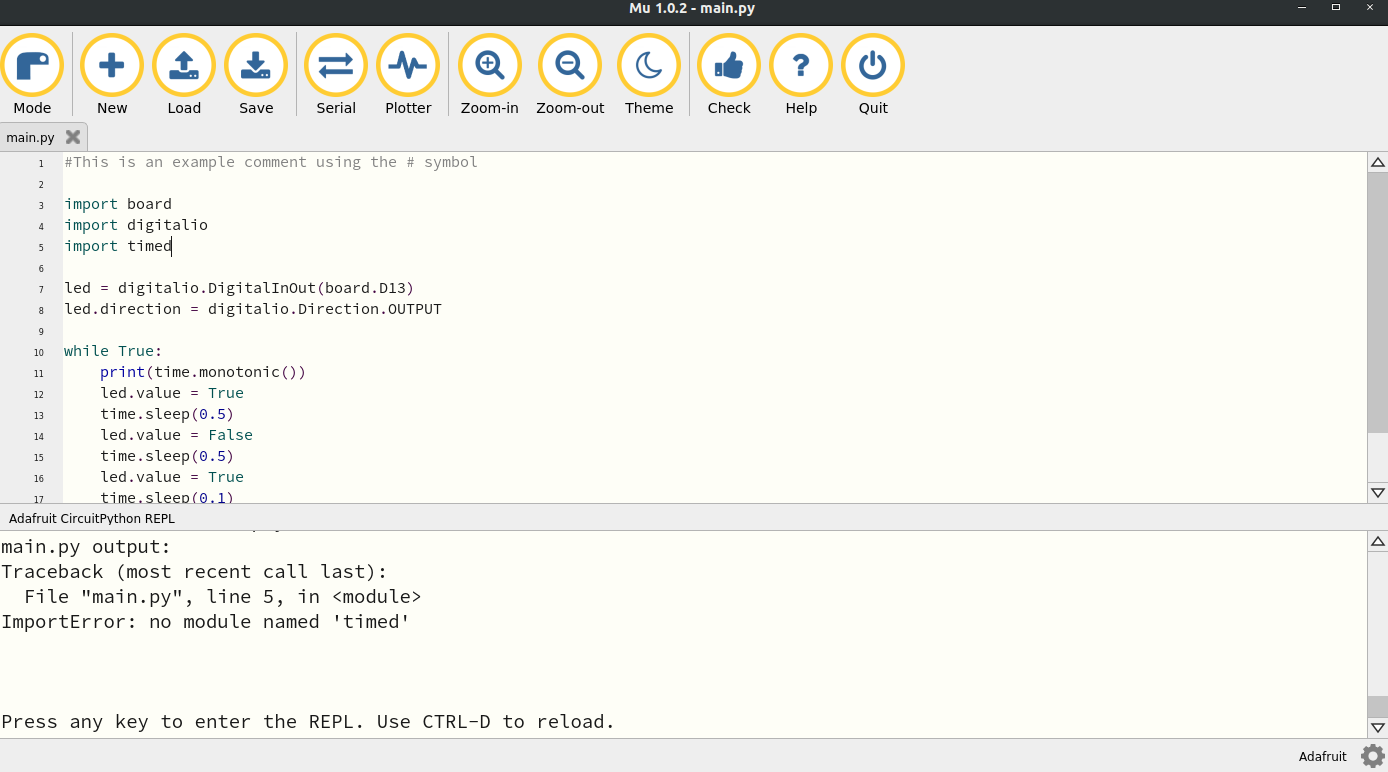
\includegraphics[width=\textwidth]{Figures/blinkerror.png}
  \end{center}
\end{figure}
In this case I have an error on line 5. It’s saying there is no module
named {\it timed}. The reason that module doesn’t exist is because the
module is actually {\it time} not {\it timed}. You can use the {\it
  Serial} monitor to check on your program and see what errors you may
have. Ok so there are two more lines of code to discuss. They are
{\it led.value = True} and {\it time.sleep(0.5)}.

These lines of code are repeated throughout the while loop and do two
things. First, the {\it led.value} either sets the value of the LED to
True which turns the light on or False which turns the light off. The
LED is digital which means the signal can either be on or off. There’s
no in between for digital signals. The {\it time.sleep()} function
tells the CPX to pause for half a second. You can change the number in
the parentheses if you want to change length of time the code
pauses. Note that the CPX completely pauses. That is no code runs
during a sleep.

If you’ve gotten the LED to blink you’re all set for this
lab. However, I’d like to you learn a few more things about
documentation. Just like Python on your desktop you can lookup the
documentation on the CPX itself. For example, I’ve added a print
statement to print the directory of time.
\begin{figure}[H]
  \begin{center}
    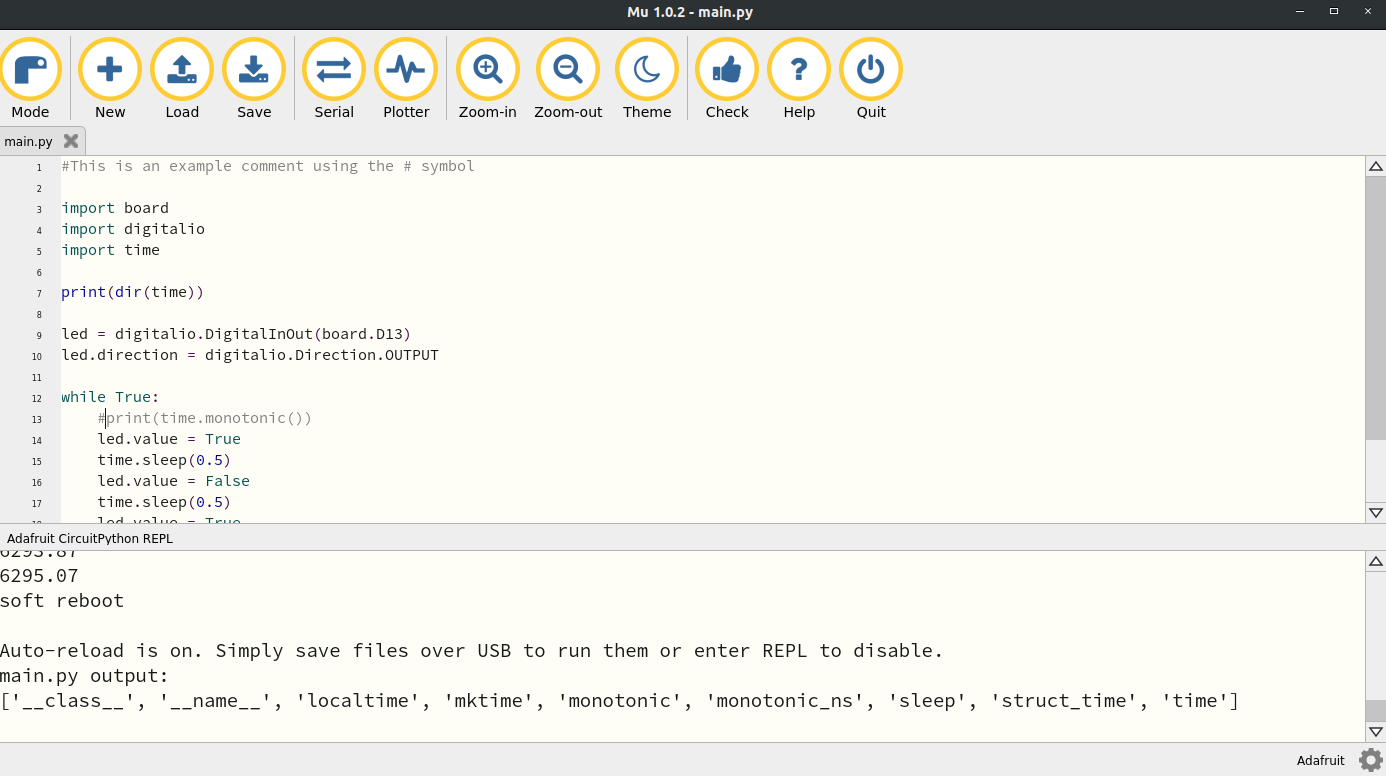
\includegraphics[width=\textwidth]{Figures/printtimeMu.png}
  \end{center}
\end{figure}
In this case I’ve added {\it print(dir(time))} to line 7. The output shows
that the {\it time} module has 9 functions including
{\it monotonic()}. Unfortunately CircuitPython does not have {\it \_\_doc\_\_}
functions built in which means if you want to learn about a specific
function, you need to visit the \href{https://circuitpython.readthedocs.io/en/5.3.x/README.html}{documentation for
CircuitPython}. Here’s the \href{https://circuitpython.readthedocs.io/en/latest/shared-bindings/time/index.html}{specific documentation for the} \href{https://circuitpython.readthedocs.io/en/latest/shared-bindings/time/index.html}{time}
\href{https://circuitpython.readthedocs.io/en/latest/shared-bindings/time/index.html}{module}. A lot of \href{https://github.com/adafruit/Adafruit_Learning_System_Guides/tree/master/CircuitPython_Essentials}{example code from the Adafruit Learning System is
also on Github.}

Finally, in order to keep practicing using Python on your desktop I
want you to modify the code above to run on your desktop
computer. You’re going to have to modify a few things. First, make
sure to open Thonny or Spyder depending on which version of Python IDE
you downloaded. Then, only import the {\it time} module. All the other
modules don’t exist on your desktop. Also, get rid of all the lines of
code that blink the LED. We just want to print time in a while
loop. Finally, the time module on your desktop uses a function called
time.time() (unless you have Python3 installed) so when you print time
make sure to use that module instead. Again visit the \href{https://docs.python.org/3/library/time.html#functions}{documentation
for time for Python if you want to learn more}. Thonny by default will
load Python version 3 but it’s possible you may have Python version 2
so make sure you look up the documentation for the appropriate version
of Python. After searching through the documentation you can use a
function called asctime() on your desktop. This is the output I get in
Thonny when I add a sleep of 1 second. The exercise for you is to do
something similar. 
\begin{figure}[H]
  \begin{center}
    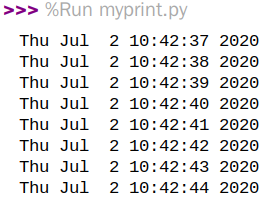
\includegraphics[width=\textwidth]{Figures/blinkcomputer.png}
  \end{center}
\end{figure}
\subsection{TL;DR}

\begin{enumerate}[itemsep=-5pt]
\item Plug in your CPX and double tap it to go into reset
  mode. CPLAYBOOT will mount to your computer. (Some CPXes you need to hold the button down instead of double tap).
\item Download the \href{https://circuitpython.org/downloads}{UF2
  file}.
\item Drag the UF2 file to your CPLAYBOOT drive. After a few seconds
  CIRCUITPY will mount.
\item You need to then download
  \href{https://codewith.mu/en/download}{Mu}
\item Open Mu and make sure to select the mode Adafruit CircuitPython (or just CircuitPython if you have a new version)
\item Open main.py (or code.py) in Mu from the CIRCUITPY drive in Mu. (It's possible you have code.py on your drive instead of main.py which is fine. Just open one or the other)
\item Copy the \href{https://github.com/cmontalvo251/Microcontrollers/blob/master/Circuit_Playground/CircuitPython/blink.py}{blink.py} script into main.py (or code.py)
\item Once you have the script running, modify the script to run on
  your Desktop using Spyder or Thonny
\end{enumerate}

There is an accompanying
\href{https://www.youtube.com/watch?v=XFvLn6rwm3I}{youtube video to
  help you see me perform the 8 steps above.}

\subsection{Assignment}

For this assignment you must appropriately set up your CPX/CPB, get the blink code to run and include some screenshots of relevant steps. {\bf Note for the blink code, modify blink pattern to be different from the default on Github}. The specific items requested are shown below.

Once you've completed the project above, upload a PDF with all of the photos and text
below included. My recommendation is for you to create a Word document
and insert all the photos and text into the document. Then export the
Word document to a PDF. For videos I suggest uploading the videos to
Google Drive, turn on link sharing and include a link in your
PDF. Note that all code must be included in the appendix or you'll be
penalized 10\%. 


\begin{enumerate}[itemsep=-5pt]
\item Include a screenshot of your computer showing the CPLAYBOOT drive on your computer - 20\%
\item Include a screenshot of your computer showing the CIRCUITPY drive on your computer - 20\%
\item Include a screenshot of Mu with the Serial monitor open showing the output of the blink code. Remember to modify the blink pattern - 20\%
\item Include a photo of your CPX with the red led on - 20\%
\end{enumerate}
